\documentclass[tikz,border=0pt]{standalone}
\pdfminorversion=7
\usepackage[T1]{fontenc}
\usepackage{lmodern,amsmath,amssymb,graphicx}
\usepackage{pgfplots}
\usetikzlibrary{arrows.meta,calc,positioning,patterns,decorations.pathreplacing}
\pgfplotsset{compat=1.18}
\definecolor{family}{RGB}{0,140,18}
\definecolor{familypale}{RGB}{225,255,226}
\definecolor{frozen}{RGB}{49,57,208}
\definecolor{frozenpale}{RGB}{234,235,255}
\definecolor{adapter}{RGB}{219,102,0}
\definecolor{adapterpale}{RGB}{255,196,135}
\definecolor{outputcol}{RGB}{120,38,130}
\definecolor{ink}{RGB}{33,33,33}
\definecolor{muted}{RGB}{105,105,105}
\tikzset{
 figure/.style={x=1pt,y=1pt,line cap=round,line join=round,text=ink,
   >={Stealth[length=7pt,width=6pt]},font=\fontsize{20}{24}\selectfont},
 title/.style={font=\fontsize{29}{33}\selectfont},
 heading/.style={font=\fontsize{22}{26}\selectfont},
 labeltext/.style={font=\fontsize{18}{22}\selectfont,align=center},
 smalllabel/.style={font=\fontsize{15}{19}\selectfont,align=center},
 equation/.style={font=\fontsize{24}{29}\selectfont,align=center},
 flow/.style={->,line width=1.3pt},
 fineflow/.style={->,line width=.8pt},
 target/.style={circle,fill=family,draw=white,line width=1.2pt,inner sep=0pt,minimum size=12pt},
 candidate/.style={circle,fill=white,draw=muted,line width=1.3pt,inner sep=0pt,minimum size=10pt},
 neuron/.style={circle,draw=frozen,fill=frozen!18,minimum size=13pt,inner sep=0pt,line width=.8pt}
}
\DeclareMathOperator{\rank}{rank}
\DeclareMathOperator{\row}{row}
\DeclareMathOperator{\col}{col}
\newcommand{\R}{\mathbb R}
\graphicspath{{assets/}}
\newcommand{\canvas}[1]{\path[use as bounding box] (0,0) rectangle (960,600);
  \node[title,anchor=west] at (36,557) {#1};}
\newcommand{\glyphgrid}[2]{
 \begin{scope}[shift={(#1,#2)}]
  \fill[white] (0,0) rectangle (136,136);
  \foreach \x/\y/\c in {1/1/80,2/2/80,2/3/45,3/4/45,3/5/45,4/5/100,4/6/45,5/6/45,5/4/45,5/2/100,6/1/80}{
    \fill[frozen!\c] (\x*17,\y*17) rectangle ++(17,17);
  }
  \draw[step=17pt,black!30,line width=.35pt] (0,0) grid (136,136);
  \draw[black!45,line width=.6pt] (0,0) rectangle (136,136);
 \end{scope}}

\begin{document}
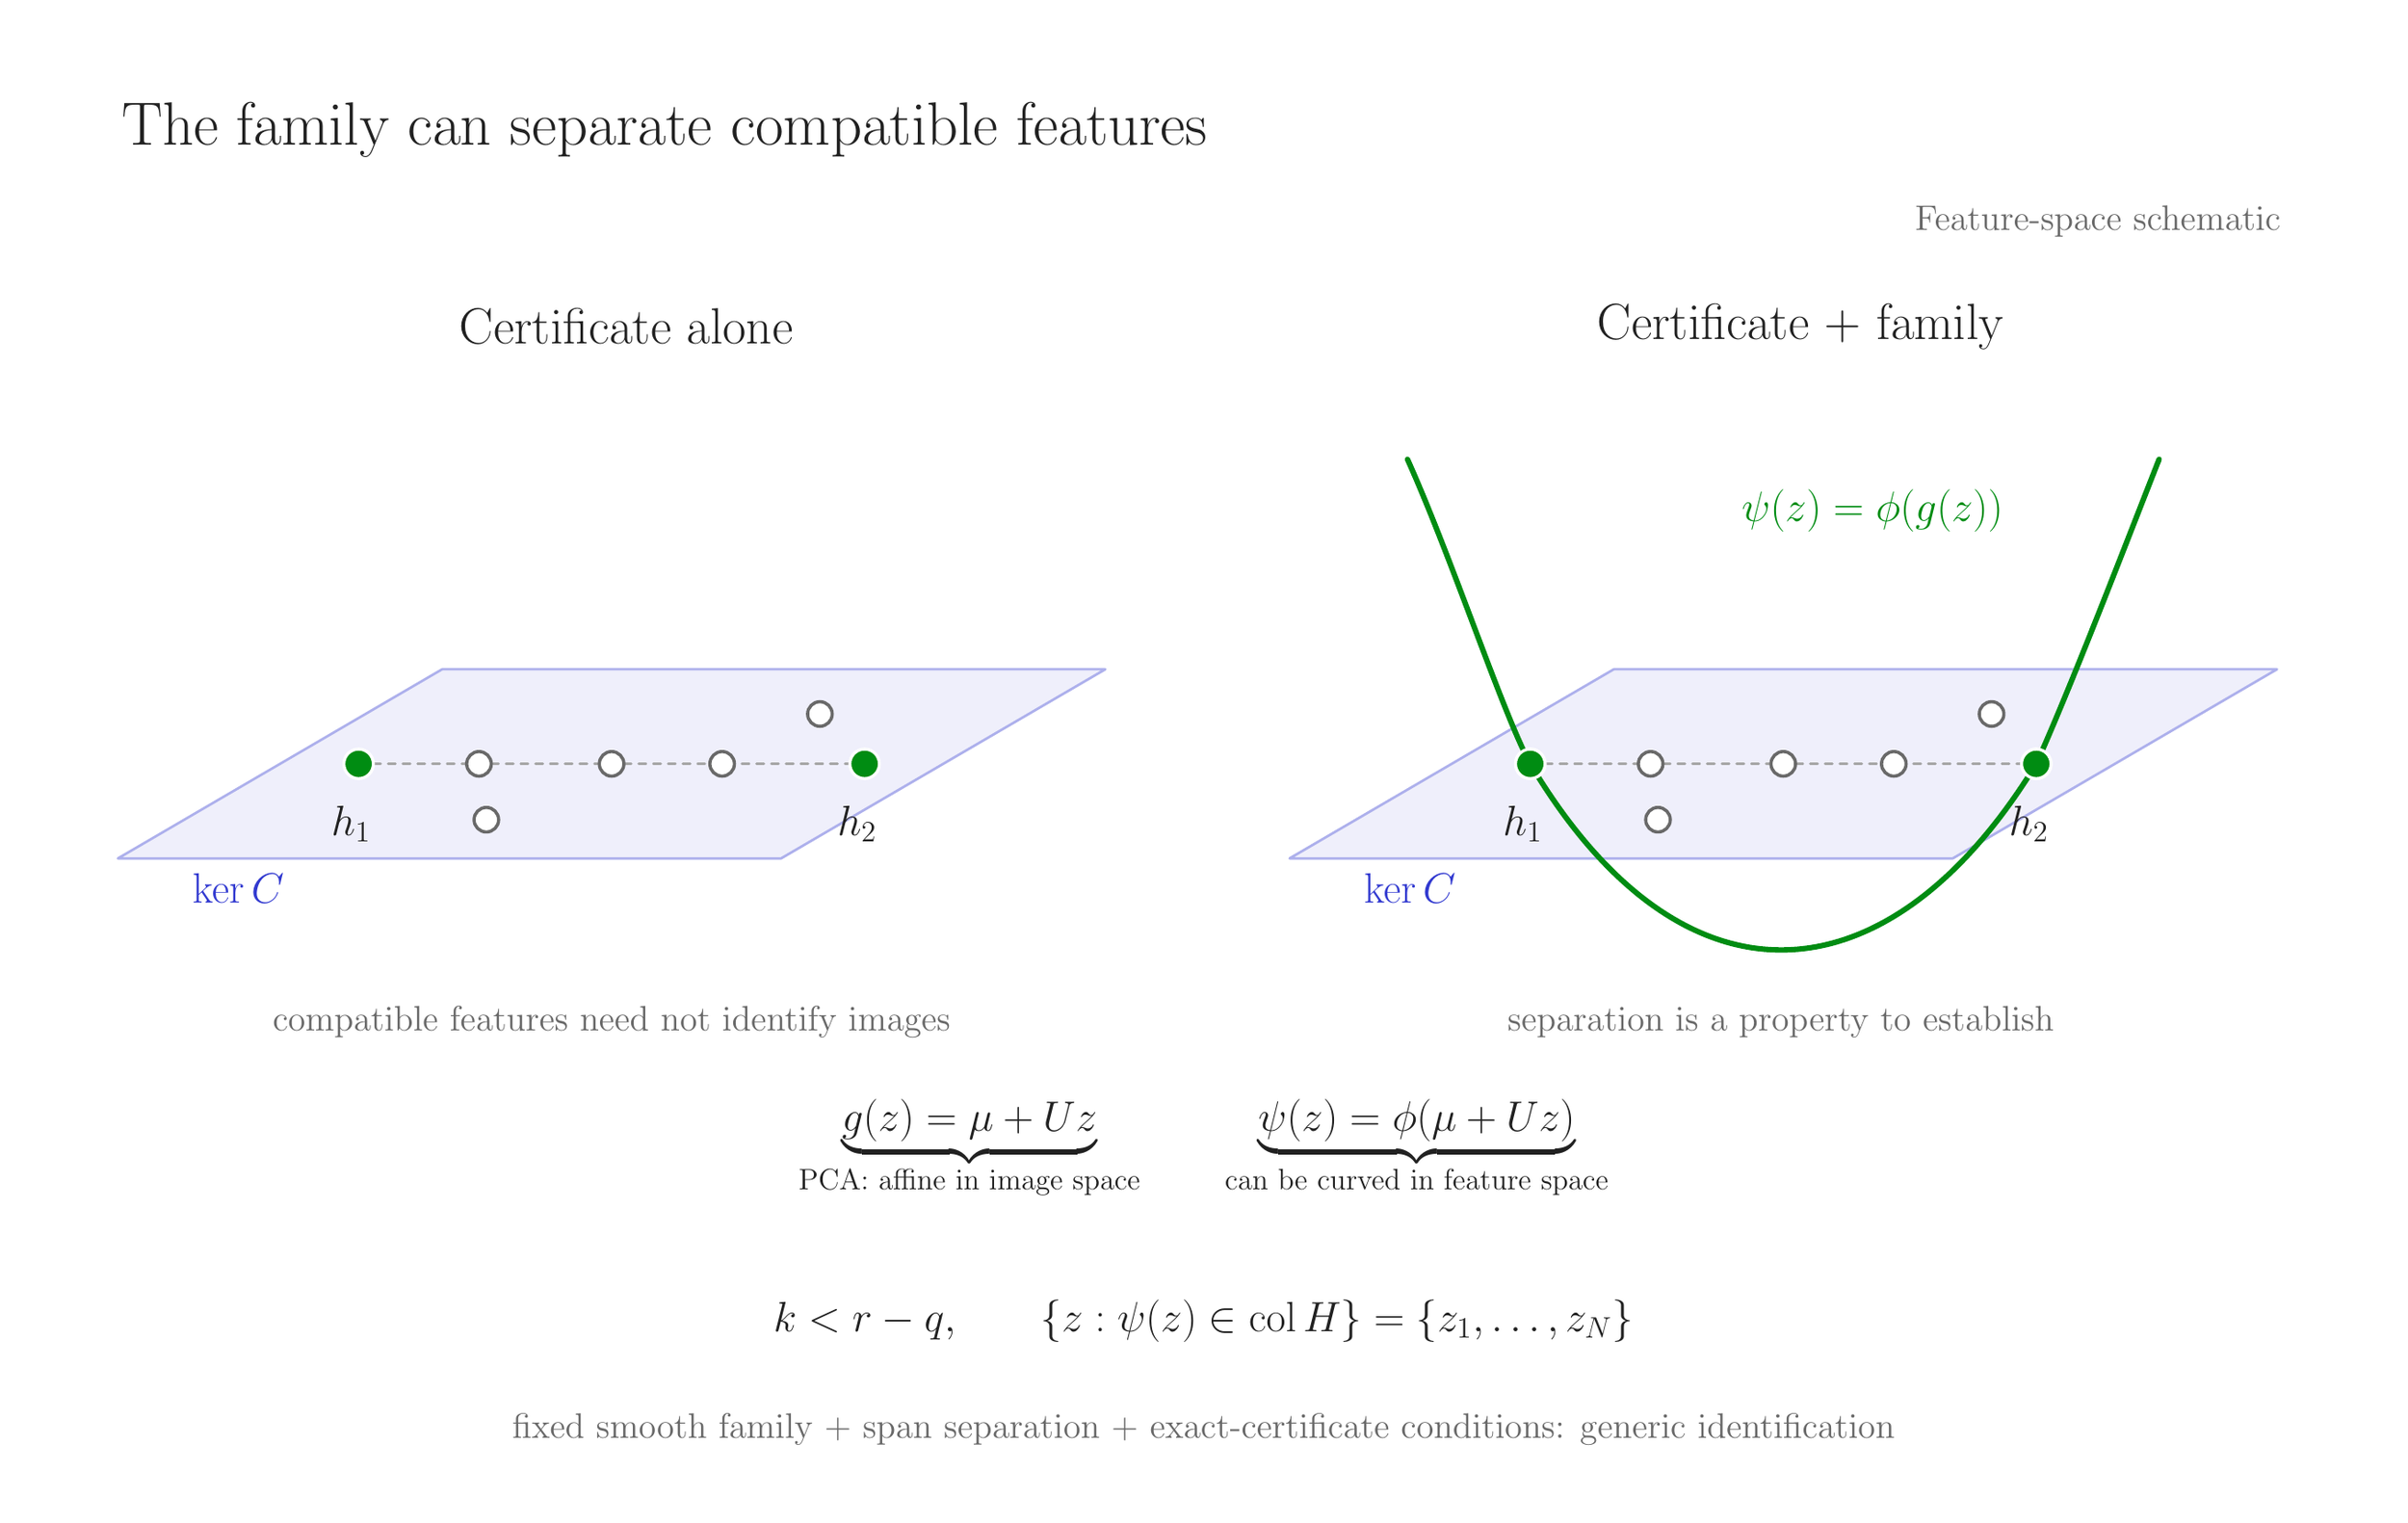
\begin{tikzpicture}[figure]
\canvas{The family can separate compatible features}
\node[smalllabel,text=muted,anchor=east] at (922,520) {Feature-space schematic};
\node[heading] at (245,477) {Certificate alone};
\node[heading] at (723,477) {Certificate $+$ family};
\foreach \xx in {239,716}{
 \begin{scope}[shift={(\xx,299)},x={(1pt,0pt)},y={(.6pt,.35pt)},z={(0pt,1pt)}]
  \filldraw[fill=frozen!8,draw=frozen!40,line width=1pt]
   (-135,-110,0)--(135,-110,0)--(135,110,0)--(-135,110,0)--cycle;
  \draw[dashed,black!35,line width=1pt] (-103,0,0)--(103,0,0);
  \node[candidate] at (-54,0,0) {};
  \node[candidate] at (0,0,0) {};
  \node[candidate] at (45,0,0) {};
  \node[candidate] at (50,58,0) {};
  \node[candidate] at (-12,-65,0) {};
  \node[target] at (-103,0,0) {};
  \node[target] at (103,0,0) {};
  \node[labeltext,anchor=north] at (-103,-5,-12) {$h_1$};
  \node[labeltext,anchor=north] at (103,-5,-12) {$h_2$};
  \node[labeltext,text=frozen] at (-65,-145,0) {$\ker C$};
 \end{scope}
}
\begin{scope}[shift={(716,299)}]
 \draw[draw=family,line width=2.2pt]
  (-153,124) .. controls (-135,84) and (-114,20) .. (-103,0)
  .. controls (-41,-104) and (43,-98) .. (103,0)
  .. controls (117,31) and (140,91) .. (153,124);
 \node[target] at (-103,0) {};
 \node[target] at (103,0) {};
 \node[labeltext,text=family,anchor=east] at (93,103) {$\psi(z)=\phi(g(z))$};
\end{scope}
\node[smalllabel,text=muted] at (239,194) {compatible features need not identify images};
\node[smalllabel,text=muted] at (715,194) {separation is a property to establish};
\node[labeltext] at (480,142) {$\underbrace{g(z)=\mu+Uz}_{\text{PCA: affine in image space}}\qquad
 \underbrace{\psi(z)=\phi(\mu+Uz)}_{\text{can be curved in feature space}}$};
\node[labeltext] at (480,72) {$k<r-q,\qquad
 \{z:\psi(z)\in\col H\}=\{z_1,\ldots,z_N\}$};
\node[smalllabel,text=muted] at (480,28) {fixed smooth family $+$ span separation $+$ exact-certificate conditions: generic identification};
\end{tikzpicture}
\end{document}
